\chapter[Introdução]{Introdução}
\label{ch:introdução}

Escreva aqui seu capítulo introdutório. Ele pode conter figuras, tabelas e subseções. Exemplo de uma citação indireta \cite{yu2011new}, e da \autoref{fig:rede_convencional}. Imagens do autor, tem na fonte o texto "Elaborado pelo autor".

% \begin{figure}[h!]
% 	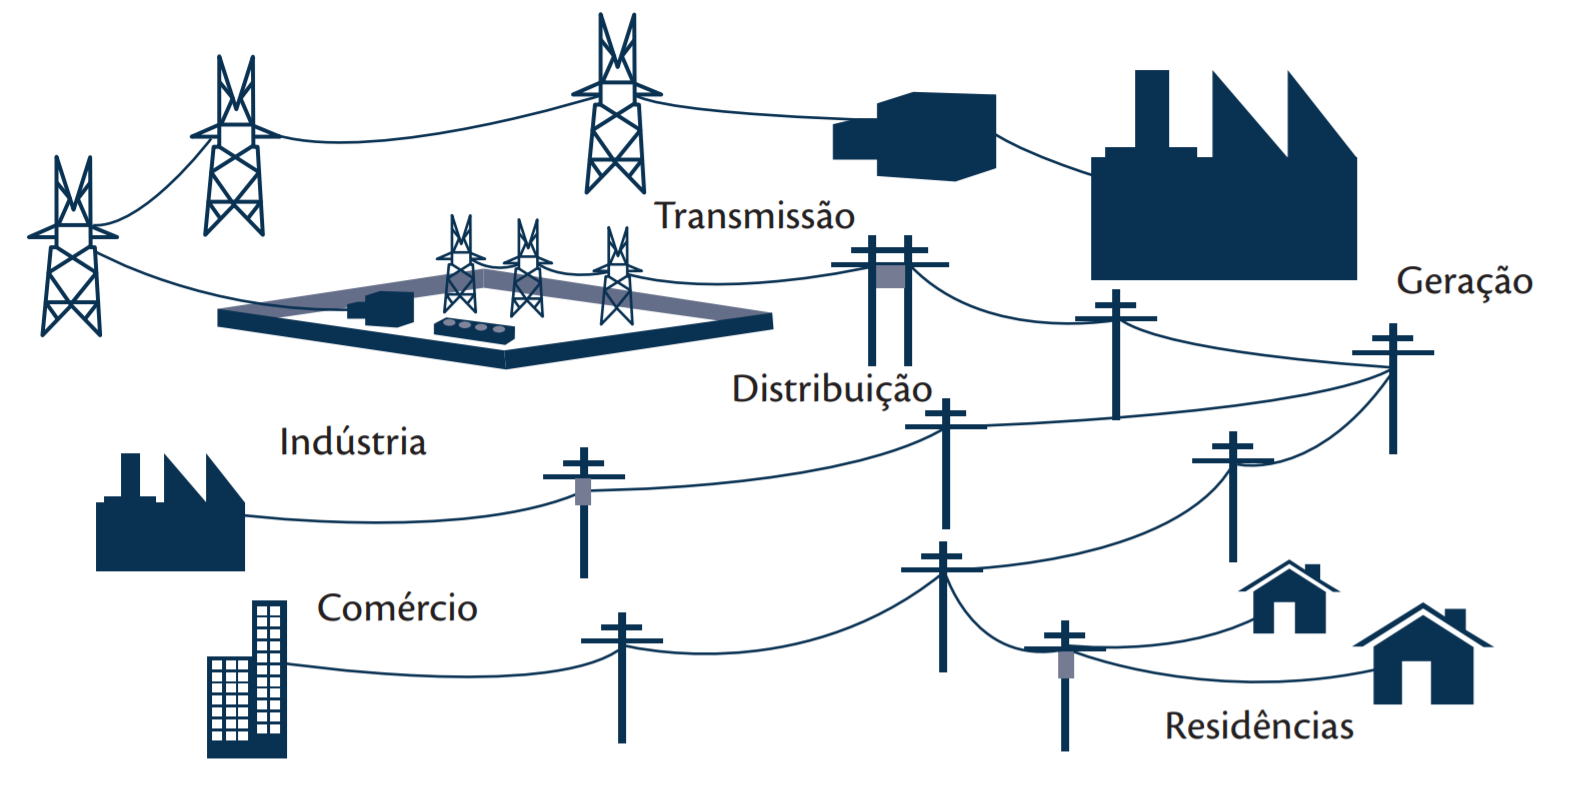
\includegraphics[width=0.9\textwidth, keepaspectratio=true]{rede_convencional}
% 	\centering
% 	\caption[Esquemático de uma rede elétrica convencional.]{Esquemático de uma rede elétrica convencional.}
% 	\fonte{\cite[p. 15]{cgee}.}
% 	\label{fig:rede_convencional}
% \end{figure}
% \FloatBarrier

Exemplo de citação direta com menos de três linhas. Como "o mercado de energia elétrica está baseado em tarifas fixas e limitações de informações em tempo real sobre gerenciamento da rede e da carga" \cite[p. 15]{cgee}, o consumidor acaba, então, não tendo como optar por fornecimentos elétricos mais adequados.


\section{Uma subseção explicativa}

Lorem ipsum, uma citação direta 

\begin{citacao}[brazil]
[...] redes elétricas que podem, de forma inteligente, integrar o comportamento e as ações de todos os usuários conectados a ela, como geradores, consumidores e os que desempenham as duas funções, para entregar, eficientemente, um fornecimento de eletricidade sustentável, econômico e seguro \cite[p. 51, tradução livre]{yu2011new}.
\end{citacao}

Para compreender melhor as grandes mudanças e os benefícios gerados pelas \textit{Smart Grids} no contexto do fornecimento elétrico, a \autoref{tab-comparativa} traz um breve comparativo entre as redes tradicionais e as redes inteligentes.

\begin{table}[!ht]
\centering
\resizebox{\textwidth}{!}{%
\begin{tabular}{ll}
\hline
\multicolumn{1}{c}{\textbf{Redes Elétricas Tradicionais}} & \multicolumn{1}{c}{\textbf{Redes Elétricas Inteligentes}}                 \\ \hline
\rowcolor[HTML]{DDDDDD} 
Eletromecânica, estado sólido                             & Digital/Microprocessadores                                                \\
Unidirecional e localmente bidirecional                   & Global/comunicação bidirecional integrada                                 \\
\rowcolor[HTML]{DDDDDD} 
Geração centralizada                                      & Acomoda geração distribuída                                               \\
{Controle, monitoramento e proteção limitados}  & WAMPAC, proteção adaptativa \\
\rowcolor[HTML]{DDDDDD} 
"Cega"                                                    & Auto-monitoramento                                                        \\
Recuperação manual                                        & Auto-reconfigurável                                                       \\
\rowcolor[HTML]{DDDDDD} 
Checagem manual de equipamentos                           & Monitoração remota de equipamentos                                        \\
Sistema de controle de contingências limitado             & Sistema de controle pervasivo                                             \\
\rowcolor[HTML]{DDDDDD} 
Confiabilidade estimada                                   & Confiabilidade preditiva                                                 
\end{tabular}%
}
\caption{Comparação entre redes elétricas convencionais e redes elétricas inteligentes}
\label{tab-comparativa}
\fonte{\cite[p. 28, tradução nossa]{ali2013smart}}
\end{table}

\section{Trabalhos Relacionados}
\lipsum[1-1]

\section{Motivação}
O que lhe motiva a realizar este trabalho.

\section{Objetivos}
Objetivo geral e específicos.

\section{Estrutura do Trabalho}
Este trabalho apresenta uma introdução sobre o tema, mostrando os fatores que motivam a implantação da ideia, além da justificativa e dos objetivos. Em sequência, o \autoref{ch:cap2} aborda (...). O \autoref{ch:cap3}, por sua vez, explica a metodologia para ..., enquanto o \autoref{ch:cap4} trata de (...). O \autoref{ch:cap5} apresenta (...). Por fim, o \autoref{ch:cap6} traz as principais conclusões e contribuições deste trabalho.
